
%(BEGIN_QUESTION)
% Copyright 2007, Tony R. Kuphaldt, released under the Creative Commons Attribution License (v 1.0)
% This means you may do almost anything with this work of mine, so long as you give me proper credit

Suppose we wish to measure water level in this vessel, where the LRV and URV points are both between the extreme limits of ``empty'' and ``full'':

$$\includegraphics[width=15.5cm]{i02963x01.eps}$$

Complete the following calibration table for this level transmitter:

% No blank lines allowed between lines of an \halign structure!
% I use comments (%) instead, so that TeX doesn't choke.

$$\vbox{\offinterlineskip
\halign{\strut
\vrule \quad\hfil # \ \hfil & 
\vrule \quad\hfil # \ \hfil & 
\vrule \quad\hfil # \ \hfil & 
\vrule \quad\hfil # \ \hfil \vrule \cr
\noalign{\hrule}
%
% First row
Process & Percent of & Hydrostatic & Output signal \cr
%
% Another row
level (in) & span (\%) & pressure (PSI) & ideal (mA) \cr
%
\noalign{\hrule}
%
% Another row
  & 0 &  &  \cr
%
\noalign{\hrule}
%
% Another row
  & 25 &  &  \cr
%
\noalign{\hrule}
%
% Another row
  & 50 &  &  \cr
%
\noalign{\hrule}
%
% Another row
  & 75 &  &  \cr
%
\noalign{\hrule}
%
% Another row
  & 100 &  &  \cr
%
\noalign{\hrule}
} % End of \halign 
}$$ % End of \vbox

\underbar{file i02963}
%(END_QUESTION)





%(BEGIN_ANSWER)

% No blank lines allowed between lines of an \halign structure!
% I use comments (%) instead, so that TeX doesn't choke.

$$\vbox{\offinterlineskip
\halign{\strut
\vrule \quad\hfil # \ \hfil & 
\vrule \quad\hfil # \ \hfil & 
\vrule \quad\hfil # \ \hfil & 
\vrule \quad\hfil # \ \hfil \vrule \cr
\noalign{\hrule}
%
% First row
Process & Percent of & Hydrostatic & Output signal \cr
%
% Another row
level (in) & span (\%) & pressure (PSI) & ideal (mA) \cr
%
\noalign{\hrule}
%
% Another row
48 & 0 & 1.734 & 4 \cr
%
\noalign{\hrule}
%
% Another row
58.5 & 25 & 2.113 & 8 \cr
%
\noalign{\hrule}
%
% Another row
69  & 50 & 2.493 & 12 \cr
%
\noalign{\hrule}
%
% Another row
79.5 & 75 & 2.872 & 16 \cr
%
\noalign{\hrule}
%
% Another row
90 & 100 & 3.251 & 20 \cr
%
\noalign{\hrule}
} % End of \halign 
}$$ % End of \vbox


%(END_ANSWER)





%(BEGIN_NOTES)


%INDEX% Measurement, level: hydrostatic pressure

%(END_NOTES)


